%%
%% This is file `sample-authordraft.tex',
%% generated with the docstrip utility.
%%
%% The original source files were:
%%
%% samples.dtx  (with options: `authordraft')
%% 
%% IMPORTANT NOTICE:
%% 
%% For the copyright see the source file.
%% 
%% Any modified versions of this file must be renamed
%% with new filenames distinct from sample-authordraft.tex.
%% 
%% For distribution of the original source see the terms
%% for copying and modification in the file samples.dtx.
%% 
%% This generated file may be distributed as long as the
%% original source files, as listed above, are part of the
%% same distribution. (The sources need not necessarily be
%% in the same archive or directory.)
%%
%% Commands for TeXCount
%TC:macro \cite [option:text,text]
%TC:macro \citep [option:text,text]
%TC:macro \citet [option:text,text]
%TC:envir table 0 1
%TC:envir table* 0 1
%TC:envir tabular [ignore] word
%TC:envir displaymath 0 word
%TC:envir math 0 word
%TC:envir comment 0 0
%%
%%
%% The first command in your LaTeX source must be the \documentclass command.
\documentclass[sigconf,authordraft]{acmart}
%% NOTE that a single column version may required for 
%% submission and peer review. This can be done by changing
%% the \doucmentclass[...]{acmart} in this template to 
%% \documentclass[manuscript,screen]{acmart}
%% 
%% To ensure 100% compatibility, please check the white list of
%% approved LaTeX packages to be used with the Master Article Template at
%% https://www.acm.org/publications/taps/whitelist-of-latex-packages 
%% before creating your document. The white list page provides 
%% information on how to submit additional LaTeX packages for 
%% review and adoption.
%% Fonts used in the template cannot be substituted; margin 
%% adjustments are not allowed.

%%
%% \BibTeX command to typeset BibTeX logo in the docs
\AtBeginDocument{%
  \providecommand\BibTeX{{%
    \normalfont B\kern-0.5em{\scshape i\kern-0.25em b}\kern-0.8em\TeX}}}

%% Rights management information.  This information is sent to you
%% when you complete the rights form.  These commands have SAMPLE
%% values in them; it is your responsibility as an author to replace
%% the commands and values with those provided to you when you
%% complete the rights form.
\setcopyright{acmlicensed}
\copyrightyear{2024}
\acmYear{2024}
\acmDOI{XXXXXXX.XXXXXXX}

%% These commands are for a PROCEEDINGS abstract or paper.
\acmConference[Conf 2024]{Conference name and year}{Date}{Place}
%
%  Uncomment \acmBooktitle if th title of the proceedings is different
%  from ``Proceedings of ...''!
%
%\acmBooktitle{Woodstock '18: ACM Symposium on Neural Gaze Detection,
%  June 03--05, 2018, Woodstock, NY} 
\acmISBN{XXX-X-XXXX-XXXX-X/XX/XX}


%%
%% Submission ID.
%% Use this when submitting an article to a sponsored event. You'll
%% receive a unique submission ID from the organizers
%% of the event, and this ID should be used as the parameter to this command.
%%\acmSubmissionID{123-A56-BU3}

%%
%% For managing citations, it is recommended to use bibliography
%% files in BibTeX format.
%%
%% You can then either use BibTeX with the ACM-Reference-Format style,
%% or BibLaTeX with the acmnumeric or acmauthoryear sytles, that include
%% support for advanced citation of software artefact from the
%% biblatex-software package, also separately available on CTAN.
%%
%% Look at the sample-*-biblatex.tex files for templates showcasing
%% the biblatex styles.
%%

%%
%% For managing citations, it is recommended to use bibliography
%% files in BibTeX format.
%%
%% You can then either use BibTeX with the ACM-Reference-Format style,
%% or BibLaTeX with the acmnumeric or acmauthoryear sytles, that include
%% support for advanced citation of software artefact from the
%% biblatex-software package, also separately available on CTAN.
%%
%% Look at the sample-*-biblatex.tex files for templates showcasing
%% the biblatex styles.
%%

%%
%% The majority of ACM publications use numbered citations and
%% references.  The command \citestyle{authoryear} switches to the
%% "author year" style.
%%
%% If you are preparing content for an event
%% sponsored by ACM SIGGRAPH, you must use the "author year" style of
%% citations and references.
%% Uncommenting
%% the next command will enable that style.
\citestyle{acmauthoryear}

%%
%% end of the preamble, start of the body of the document source.
\usepackage{url} % To handle \url
\usepackage{hyperref} % For clickable URLs
\begin{document}

%%
%% The "title" command has an optional parameter,
%% allowing the author to define a "short title" to be used in page headers.
\title{MFCCs, Chroma Features, and Spectrogram Images for Deepfake Audio Classification Using Machine Learning}

%%
%% The "author" command and its associated commands are used to define
%% the authors and their affiliations.
%% Of note is the shared affiliation of the first two authors, and the
%% "authornote" and "authornotemark" commands
%% used to denote shared contribution to the research.
\author{Nora Bakken, Shavil Singh, Makwana Prashant Lnu, and Tapadhir Das}
\affiliation{%
  \institution{Department of Computer Science, University of the Pacific}
  \streetaddress{3601 Pacific Ave}
  \city{Stockton}
  \state{California}
  \country{USA}
  \postcode{95211-0110}
}
\email{n_bakken@u.pacific.edu, tdas@pacific.edu}
\orcid{XXXX-XXXX-XXXX-XXXX}



%%
%% By default, the full list of authors will be used in the page
%% headers. Often, this list is too long, and will overlap
%% other information printed in the page headers. This command allows
%% the author to define a more concise list
%% of authors' names for this purpose.
\renewcommand{\shortauthors}{Bakken, Singh, \& Lnu, et al.}

%%
%% The abstract is a short summary of the work to be presented in the
%% article.
\begin{abstract}

\end{abstract}

%%
%% The code below is generated by the tool at http://dl.acm.org/ccs.cfm.
%% Please copy and paste the code instead of the example below.
%%
\begin{CCSXML}
<ccs2012>
 <concept>
<concept_id>10003456.10003457.10003527.10003531.10003533</concept_id>
<concept_desc>Social and professional topics~Machine Learning</concept_desc>
<concept_significance>300</concept_significance>
</concept>
<concept>
<concept_id>10010405.10010489.10010491</concept_id>
<concept_desc>Cybersecurity~Interactive learning environments</concept_desc>
<concept_significance>300</concept_significance>
</concept>
<concept>
<concept_id>10011007.10010940.10010941.10010969.10010970</concept_id>
<concept_desc>Adversarial attack protection~Interactive games</concept_desc>
<concept_significance>300</concept_significance>
</concept>
</ccs2012>
\end{CCSXML}

\ccsdesc[300]{Mel-frequency cepstral coefficients (MFCCs)~Audio representation}
\ccsdesc[300]{Convolutional Neural Networks~Machine Learning}
\ccsdesc[300]{Adversarial attack protection~Cybersecurity}

%%
%% Keywords. The author(s) should pick words that accurately describe
%% the work being presented. Separate the keywords with commas.
\keywords{MFCCs, Spectrogram, VGG16, ResNet50, Chroma Features, SVM, Gradient Boosting, Deepfakes}

\received{XX December 2024}
\received[revised]{XX X XXXX}
\received[accepted]{X X XXXX}

%%
%% This command processes the author and affiliation and title
%% information and builds the first part of the formatted document.
\maketitle

\section{Introduction}

\section{Motivation}

With the rise of artificial intelligence (AI), deepfakes are more prevalent than ever, bringing with them a slough of potential dangers in a variety of areas. Likely the most well-known effect of deepfakes in everyday life is the rise of false media, especially targeting individuals. 

The American Bar Association highlighted a targeted defamation attack involving an audio recording with the voice of a high school principal making racist and antisemitic comments. After the recording spread throughout the school, the principal was in danger of losing his livelihood. He denied making these comments. After a thorough investigation, the local police deemed the recording to have been manipulated using AI \cite{b5}. 

The less talked about consequence of accessible and easy to create deepfakes is the rise of non-consensual explicit deepfake attacks on individuals. These attacks, along with being traumatic to the individual, are expanding the ever-present gender gap at the global level, inflicting consequences at the societal level \cite{b3}.

In the recent United States election, nearly half of American voters stated that deepfakes had an influence on their ballots \cite{b1}. Looking at this problem from a purely monetary perspective, CFO states that 92 percent of companies have experienced financial loss due to a deepfake \cite{b4}. This is a significant economic impact. 

These are just a few of many examples of individuals who have been hurt by deepfake attacks. There is no question about the negative impact that deepfakes actively have on our lives. It is now imperative that an application is developed to reliably identify deepfakes so that fewer individuals are harmed. 

\section{Literature Review}

\section{System Model / Background}

Numerous technologies and algorithms were explored to gather insights on the most effective methods for deepfake audio detection. In this section we will explore the complex features we utilized in our data preprocessing pipeline and discuss the sophisticated machine learning models we employed in our experiments. 

\subsection{MFCCs}

Mel-Frequency Cepstral Coefficients, or MFCCs, are a widely used feature set for speech recognition and other audio processing applications. They are a competitive feature set because they mimic what the human ear perceives \cite{9996362}. The process of extracting MFCCs involves several steps that convert raw audio into a compact representation of its spectral characteristics. One of the key stages in this process is the de-correlation of the log energies from a filter bank. The following quote provides a more detailed explanation of how MFCC coefficients are derived:

\begin{quote}
  "MFCC coefficients are obtained by de-correlating the output log
  energies of a filter bank which consists of triangular filters, linearly spaced on the Mel frequency scale.
  Conventionally an implementation of discrete cosine transform (DCT) known as distributed DCT (DCT - II) is
  used to de-correlate the speech as it is the best available approximation of the Karhunen-Loeve Transform
  (KLT)" \cite{5709752}.
\end{quote}

The resulting vector represents spectral acoustic features as floating-point numbers. These values capture essential characteristics of the audio that aid the model in distinguishing between real and fake samples. The vector's size is flexible and depends on user configuration. 

Generating a vector of MFCC features was an essential step in our preprocessing efforts. A sample rate of 44100 Hz corresponding to a maximum sound frequency of 22050 Hz is usually used for recording sound, because a human can hear sounds ranging from 20 Hz to 20000 Hz \cite{9252126}. In our experiments, we used a sampling rate of 22050 Hz. This is half of the common sample rate for recording sound, and is a common value for sampling rate when generating MFCCs. This resulted in 20 features for each audio sample. These features were then saved to a CSV file, making them available for later model training. These features played a pivotal role in the model's ability to make accurate decisions.

\subsection{Mel-Spectrogram Images}
A Mel-Spectrogram image is an alternative method for visually representing sound. Generally, we see sound visualized as a two-dimensional waveform showing amplitude over time. Figure~\ref{fig:real_waveform} shows an example of a "real" audio sample as a commonly seen waveform. Conversely, figure~\ref{fig:fake_waveform} shows an example of a "fake" audio sample as a waveform. While these representations are helpful, they do not provide enough information for a model to be able to make a decision. 

A spectrogram is a representation of an audio signal as its frequency spectrum varies over time. Similar to MFCCs, Mel-Spectrograms are generated by performing a number of transformations on an audio sample, then representing the results as a graph. First, the audio is divided into short segments of time. We used approximately 93 ms segments. Then, a Hamming window is applied to each segment.

The Hamming window can be found with the following formula \cite{9252126}:
\begin{equation}
w(n) = \alpha_0 - (1 - \alpha_0) \cos\left(\frac{2\pi n}{N-1}\right), \quad 0 \leq n \leq N-1
\end{equation}
where \(\alpha_0 = \frac{25}{46}\), and \(N\) is the window length.

Following this operation, Fast Fourier transform (FFT) is applied to calculate the power spectrum of each frame. Lastly, we can obtain the Mel-Spectrogram by applying the Mel filter bank. Frequencies are convered to the Mel scale using the following formula \cite{9252126}:
\begin{equation}
\text{mel} = 2595 \, \lg\left(1 + \frac{f}{700}\right)
\end{equation}

\begin{figure}
  \centering
  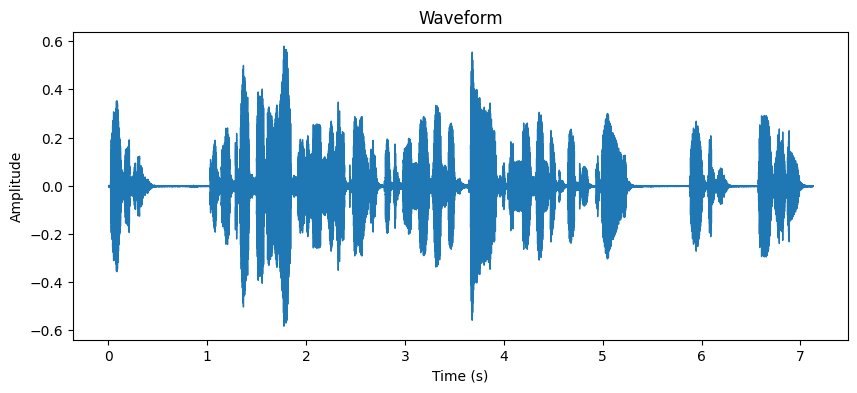
\includegraphics[width=\linewidth]{images/real_waveform.png}
  \caption{Waveform representation of a Real Audio Sample.}
  \label{fig:real_waveform}
\end{figure}

\begin{figure}
  \centering
  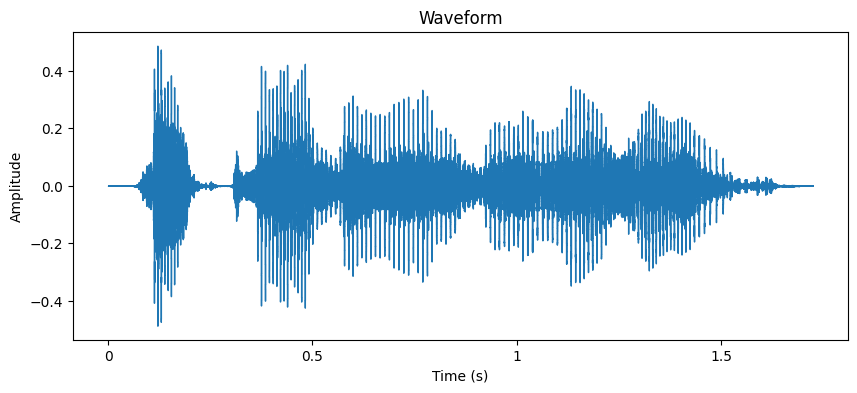
\includegraphics[width=\linewidth]{images/fake_waveform.png}
  \caption{Waveform representation of a Fake Audio Sample.}
  \label{fig:fake_waveform}
\end{figure}

\begin{figure}
  \centering
  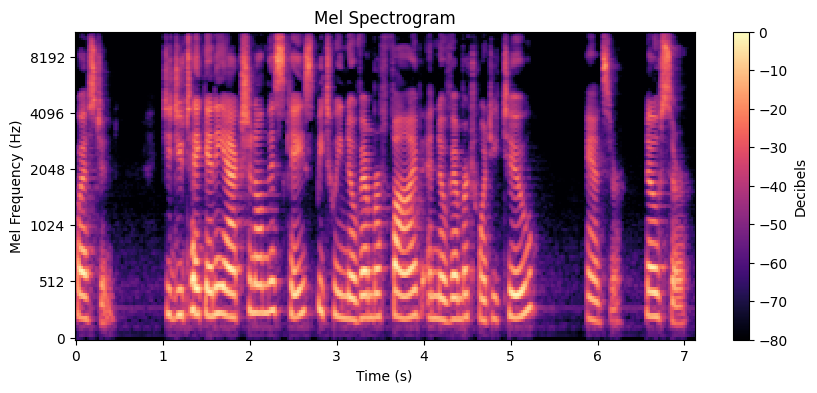
\includegraphics[width=\linewidth]{images/real_spectrogram.png}
  \caption{Spectrogram representation of a Real Audio Sample.}
  \label{fig:real_spectrogram}
\end{figure}

\begin{figure}
  \centering
  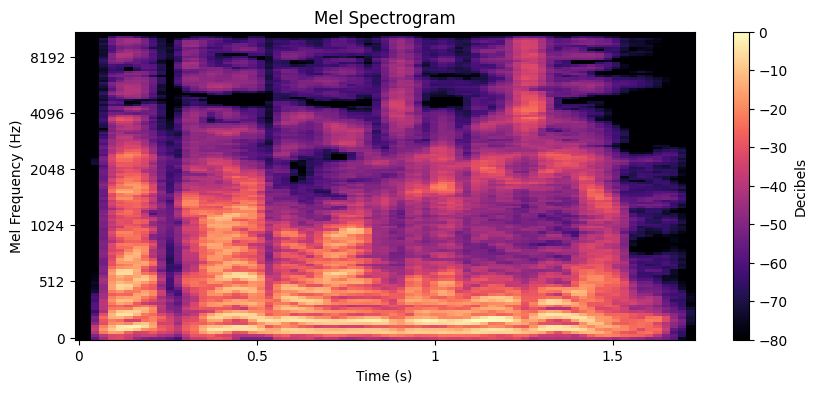
\includegraphics[width=\linewidth]{images/fake_spectrogram.png}
  \caption{Spectrogram representation of a Fake Audio Sample.}
  \label{fig:real_spectrogram}
\end{figure}


\subsection{Convolutional Neural Networks}
Nora TODO
\subsubsection{VGG16}
Nora TODO
\subsubsection{ResNet50}
Nora TODO

\subsection{Support Vector Machine (SVM)}

\subsection{Chroma Features}

\subsection{Gradient Boosting}

\section{Methodology}

\subsection{Probably a section about the data here would be good}

\section{Results}

\subsection{for-original dataset}

\subsection{for-norm dataset}

\subsection{for-2sec dataset}

\subsection{for-rerec dataset}

\section{Future Work}
Nora TODO
\section{Conclusion}

%%
%% The acknowledgments section is defined using the "acks" environment
%% (and NOT an unnumbered section). This ensures the proper
%% identification of the section in the article metadata, and the
%% consistent spelling of the heading.
\begin{acks}

\end{acks}

%%
%% The next two lines define the bibliography style to be used, and
%% the bibliography file.

\bibliographystyle{ACM-Reference-Format}
\bibliography{sample} % Reference to .bib file

\end{document}



%%
%% If your work has an appendix, this is the place to put it.
%% \appendix

%% \section{Research Methods}

%% \subsection{Part One}

%% Lorem ipsum dolor sit amet, consectetur adipiscing elit. Morbi

\end{document}
\endinput
%%
%% End of file `sample-authordraft.tex'.
https://www.overleaf.com/project/65e2871cae82cda8148c633d